\section{Money-metric well-being and structural inequality decomposition}\label{money-metric-well-being-and-structural-inequality-decomposition}

\subsection{The measure}\label{the-measure}

Fix a household \(i\) and a coalition state \(S\), which determines the utility index \(L_{i,S}\), the normalized opportunity density \(\widehat g_{i,S}\) and the priced consumption \(C_{i,S}\) at every package. Define the attained ex-ante value and the reference mass

\[
J_{i,S}=\int e^{L_{i,S}(j)}\left(\frac{C_{i,S}(j)}{\lambda_c}\right)^{\beta_c}\widehat g_{i,S}(j)\,d\nu(j),
\qquad
H_{i,S}=\int e^{L_{i,S}(j)}\,\widehat g_{i,S}(j)\,d\nu(j).
\]

The reference offers the same flat monthly amount \(m\) at every package while retaining that state's \(L\) and \(\widehat g\), so the value of the reference is

\[
\Phi_{i,S}(m)=\beta_c\log(m/\lambda_c)+\log H_{i,S},
\qquad \Phi_{i,S}'(m)=\beta_c/m>0 .
\]

The money metric is the amount at which the reference reaches the attained value, \(\Phi_{i,S}(W_{i,S})=\log J_{i,S}\), which inverts in closed form:

\[
\boxed{\;W_{i,S}=\lambda_c\exp\!\left[\frac{\log J_{i,S}-\log H_{i,S}}{\beta_c}\right].\;}
\]

Writing \(r_{i,S}(dj)=e^{L_{i,S}(j)}\widehat g_{i,S}(j)\,d\nu(j)/H_{i,S}\) for the reference probability measure, the same object is

\[
\boxed{\;W_{i,S}=\left[\int C_{i,S}(j)^{\beta_c}\,r_{i,S}(dj)\right]^{1/\beta_c}.\;}
\]

The measure is therefore a \textbf{weighted power mean of consumption of order \(\beta_c\)}, taken under a reference measure that weights packages by their non-consumption value and their availability. It is an arithmetic mean only at \(\beta_c=1\). The normalizer \(\lambda_c\) cancels between the two forms, which is why the constant is a units convention and not a modelling choice; we verify this numerically to a maximum relative deviation of 2.7e-15 across four widely separated values.

\begin{figure}[H]
\centering
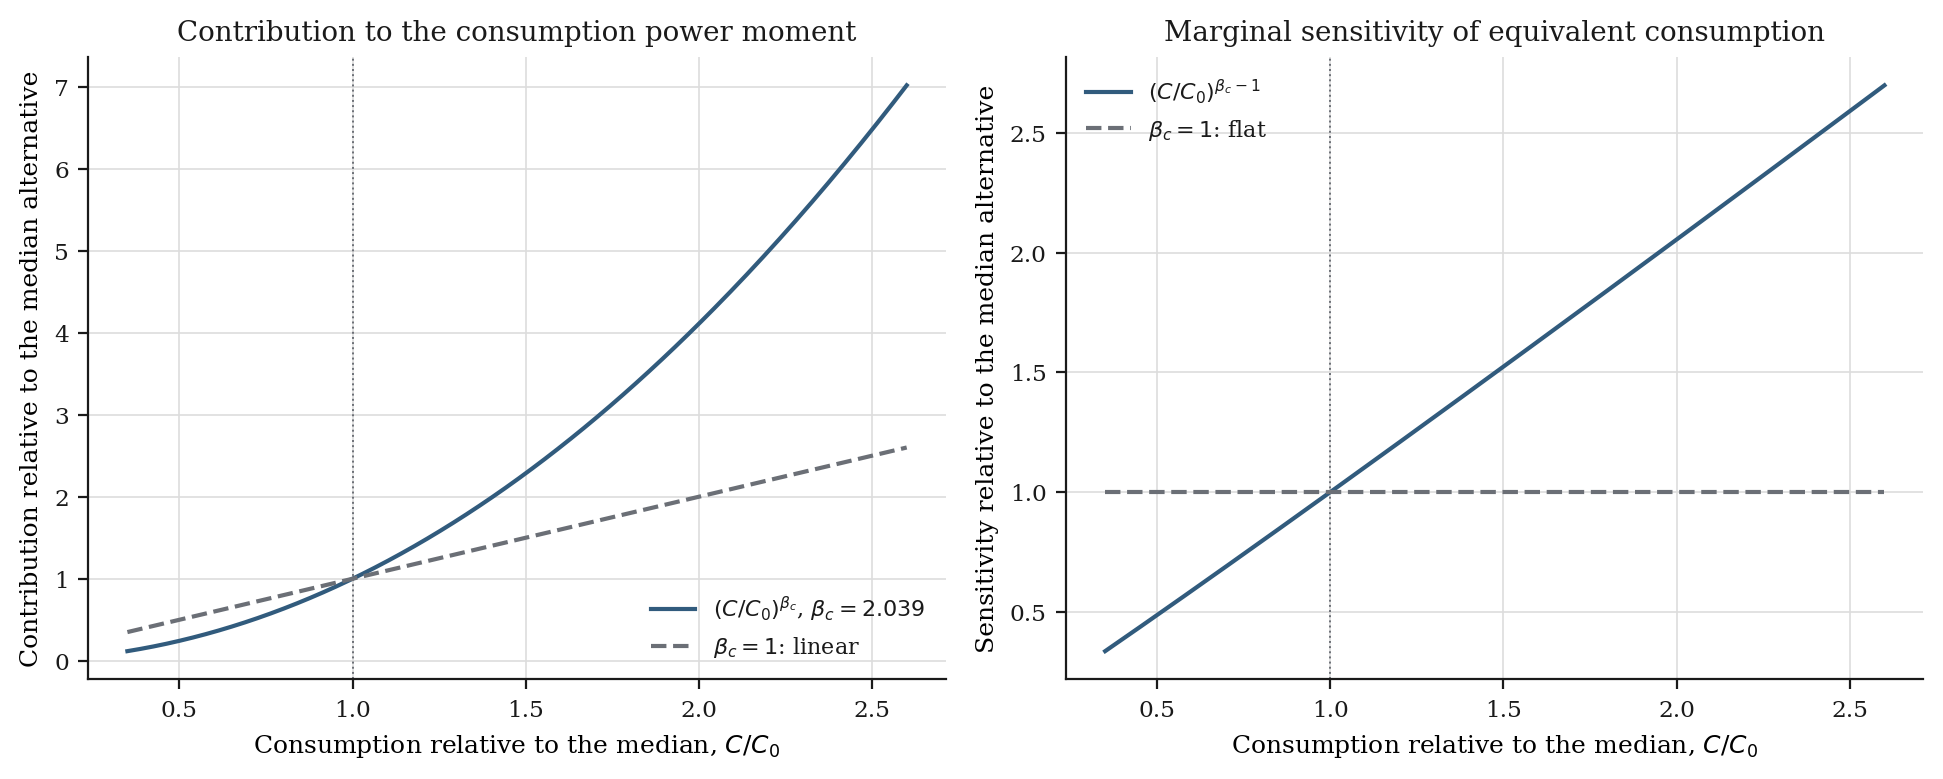
\includegraphics[width=0.95\linewidth,height=\textheight,keepaspectratio,alt={The consumption coefficient as the order of a power mean. Left: the contribution an alternative makes to the consumption power moment, relative to the median alternative, against the linear comparison at \textbackslash beta\_c=1. Right: the marginal effect of that alternative's consumption on the resulting equivalent amount, which carries exponent \textbackslash beta\_c-1, against the flat comparison at \textbackslash beta\_c=1. Neither curve is a reference probability weight: holding the reference measure fixed, those weights do not vary with consumption at all.}]{figures/v5/figV07_power_mean.png}
\caption{The consumption coefficient as the order of a power mean. Left: the contribution an alternative makes to the consumption power moment, relative to the median alternative, against the linear comparison at \(\beta_c=1\). Right: the marginal effect of that alternative's consumption on the resulting equivalent amount, which carries exponent \(\beta_c-1\), against the flat comparison at \(\beta_c=1\). Neither curve is a reference probability weight: holding the reference measure fixed, those weights do not vary with consumption at all.}
\end{figure}

Three quantities are easy to conflate and are distinct. The reference probability weight \(r_j\) does not vary with consumption at all when the reference measure is held fixed. The \emph{contribution} an alternative makes to the power moment is proportional to \(C_j^{\beta_c}\), so an alternative paying twice the median contributes 4.11 times as much at the estimated single-adult coefficient. The \emph{marginal effect} of that alternative's consumption on the resulting amount is \(\partial W/\partial C_j=r_jC_j^{\beta_c-1}W^{1-\beta_c}\), with exponent \(\beta_c-1\). The figure plots the second and the third and labels each; neither is a statement that the alternative is more available.

\(\beta_c\) is the order of this power mean and the coefficient on log consumption. It is not the consumption curvature, which is exactly zero here, and it is not an inequality-aversion parameter across households, which belongs to the index applied in Section 5 and not to the household's own aggregator.

\subsection{What the reference does and does not do to pay}\label{what-the-reference-does-and-does-not-do-to-pay}

Under the stated factorization the reference is invariant to the conditional wage density: that density integrates to one on its support and the non-consumption index has no wage argument, so replacing it leaves \(H_{i}\) unchanged. Numerically, the largest household change in \(\log H\) is 1.8e-15 for single adults and 7.1e-15 for couples, and the median change in the money metric through the direct reference channel is exactly 0 euros.

Changes in earning opportunities nevertheless change the measure, because they change what the household attains: the median total change is -17.43 euros per month for single adults and 110.53 for couples. The correct statement is therefore narrow and we make only it: \emph{the reference is directly pay-neutral, and earning opportunities reach the measure through the attained evaluation.} A total change that travels through attainment does not establish that the deterministic independence-of-pay axiom fails for this stochastic functional. That would require fixing the primitives the axiom holds fixed and proving the property, which we have not done and do not claim.

\subsection{Interpersonal comparison and the unit}\label{interpersonal-comparison-and-the-unit}

The measure is defined at the household. Comparing households of different size requires an equivalence scale, which is a normative choice and not an estimate. We report every result on two bases: a raw household basis, and an equivalized basis using the modified OECD scale. We never pool the two household types into one distribution, because the two applications carry different reference constructions and the levels are not comparable; every share below is a share of the baseline inequality of its own population.

\subsection{The structural decomposition}\label{the-structural-decomposition}

Let \(X_i=(P_i,A_i,B_i,D_i)\) collect the four structural inputs for household \(i\):

\begin{itemize}
\tightlist
\item
  \(P_i\) the arguments of the preference index: the leisure-weight covariates and the sex- or spouse-specific preference block;
\item
  \(A_i\) the arguments of job access: the employment index covariates and the occupation access table;
\item
  \(B_i\) the arguments of earning opportunities: the covariates entering the offered-wage location;
\item
  \(D_i\) the household budget inputs: non-labour resources, the roster and needs.
\end{itemize}

Let \(\mathcal I\) be an inequality index and \(W_i(\cdot)\) the money metric of the previous subsection, so that the baseline is \(I_\varnothing=\mathcal I\{W_i(X_i)\}_{i=1}^N\). For each factor define a \textbf{structural equalization operator} \(T_P,T_A,T_B,T_D\), which replaces that factor's arguments across all households by a common reference profile and leaves the estimated coefficients in place. For a coalition \(S\subseteq\{P,A,B,D\}\) let \(X^S=T_S(X)\) be the state in which exactly the factors in \(S\) are equalized, and set

\[
I_S=\mathcal I\{W_i(T_S X)\}_{i=1}^{N},
\qquad
v(S)=I_\varnothing-I_S .
\]

\(v\) is a cooperative game on four players: the worth of a coalition is the inequality it removes when its factors are equalized together. Two points about \(T_S\) are part of the economics and not of the notation. First, \(T_S\) is a single simultaneous substitution map, not an ordered product \(\prod_{k\in S}T_k\): a product is not well defined unless the operators commute on the permitted objects, and the budget operator does not commute with the others, since it reprices. Second, an operator changes a \emph{pathway}, not every occurrence of a raw characteristic. Education enters both the offered-wage location and the local-market lookup; \(T_B\) substitutes the first and leaves the second in place.

\Needspace*{12\baselineskip}\small\setlength{\tabcolsep}{3pt}\begin{longtable}[]{@{}
  >{\raggedright\arraybackslash}p{(\linewidth - 6\tabcolsep) * \real{0.2500}}
  >{\raggedright\arraybackslash}p{(\linewidth - 6\tabcolsep) * \real{0.2500}}
  >{\raggedright\arraybackslash}p{(\linewidth - 6\tabcolsep) * \real{0.2500}}
  >{\raggedright\arraybackslash}p{(\linewidth - 6\tabcolsep) * \real{0.2500}}@{}}
\caption{The four structural equalization operators. Each operator replaces the arguments of one structural pathway with a common reference profile and leaves the estimated coefficients in place; it does not equalize every occurrence of a raw characteristic. Education, for example, enters both the wage location and the local-market lookup, and only the named pathway is substituted. Operators are applied as one simultaneous substitution map, not as an ordered product.}\tabularnewline
\toprule\noalign{}
\begin{minipage}[b]{\linewidth}\raggedright
Operator
\end{minipage} & \begin{minipage}[b]{\linewidth}\raggedright
What is replaced
\end{minipage} & \begin{minipage}[b]{\linewidth}\raggedright
What is retained
\end{minipage} & \begin{minipage}[b]{\linewidth}\raggedright
Repricing
\end{minipage} \\
\midrule\noalign{}
\endfirsthead
\toprule\noalign{}
\begin{minipage}[b]{\linewidth}\raggedright
Operator
\end{minipage} & \begin{minipage}[b]{\linewidth}\raggedright
What is replaced
\end{minipage} & \begin{minipage}[b]{\linewidth}\raggedright
What is retained
\end{minipage} & \begin{minipage}[b]{\linewidth}\raggedright
Repricing
\end{minipage} \\
\midrule\noalign{}
\endhead
\bottomrule\noalign{}
\endlastfoot
\(T_P\) preferences & Singles: the arguments of the leisure weight and the complete reference-sex leisure block. Couples: the medoid spouse arguments, with own spouse coefficients retained & Budget roster, resources, access and wage pathways of the same characteristics & No: pure utility shifters do not change the budget \\
\(T_A\) job access & The arguments of the employment index and the occupation access table & Preferences, wage location, budget inputs; sex-specific occupation coefficients & No: the priced jobs are unchanged \\
\(T_B\) earning opportunities & The arguments of the offered-wage location: education shares and experience moments, with squares recomputed rather than averaged & The estimated wage coefficients and dispersion; the preference and access pathways of the same characteristics & No on a common priced node set: the change is in the density over nodes \\
\(T_D\) resources and needs & The non-labour budget inputs, the household roster and the needs profile & Every non-budget structural pathway & Yes: the household budget is recomputed through the tax-benefit system \\
\end{longtable}

Welfare and inequality are then recomputed from the model for all sixteen coalitions. There is no linearisation and no re-estimation: coefficients are held at their estimates throughout, and only the arguments move. The budget operator additionally reruns the household through the tax-benefit system, so its counterfactual consumption is priced rather than scaled.

The interactions are allocated with the \textbf{grouped Shapley--Owen--Shorrocks} rule for the partition \(\{\{P\},\{A,B,D\}\}\): the Owen value \citep{owen1977} for a game with a priori unions, applied to \(v\) in the form \citet{shorrocks2013} sets out for distributional analysis and \citet{audoly2025} document for grouped nonlinear decompositions. The grouping is chosen because the paper's question is first about preferences against circumstances and only then about which circumstance; the lower-level subdivision of \(\{A,B,D\}\) is allocated within the union. The allocation is exhaustive: the contributions sum to \(I_\varnothing-I_{\{P,A,B,D\}}\), and \(I_{\{P,A,B,D\}}\) is zero to numerical precision. We verify that closure rather than imposing it; residuals are reported in Section 5.

